%%%%%%%%%%%%%%%%%%%%%%%%%%%%%%%%%%%%%%%%%
% Beamer Presentation
% LaTeX Template
% Version 1.0 (10/11/12)
%
% This template has been downloaded from:
% http://www.LaTeXTemplates.com
%
% License:
% CC BY-NC-SA 3.0 (http://creativecommons.org/licenses/by-nc-sa/3.0/)
%
%%%%%%%%%%%%%%%%%%%%%%%%%%%%%%%%%%%%%%%%%

%----------------------------------------------------------------------------------------
%	PACKAGES AND THEMES
%----------------------------------------------------------------------------------------

\documentclass{beamer}

\mode<presentation> {

% The Beamer class comes with a number of default slide themes
% which change the colors and layouts of slides. Below this is a list
% of all the themes, uncomment each in turn to see what they look like.

%\usetheme{default}
%\usetheme{AnnArbor}
%\usetheme{Antibes}
%\usetheme{Bergen}
%\usetheme{Berkeley}
%\usetheme{Berlin}
%\usetheme{Boadilla}
%\usetheme{CambridgeUS}
%\usetheme{Copenhagen}
%\usetheme{Darmstadt}
%\usetheme{Dresden}
%\usetheme{Frankfurt}
%\usetheme{Goettingen}
%\usetheme{Hannover}
%\usetheme{Ilmenau}
%\usetheme{JuanLesPins}
%\usetheme{Luebeck}
\usetheme{Madrid}
%\usetheme{Malmoe}
%\usetheme{Marburg}
%\usetheme{Montpellier}
%\usetheme{PaloAlto}
%\usetheme{Pittsburgh}
%\usetheme{Rochester}
%\usetheme{Singapore}
%\usetheme{Szeged}
%\usetheme{Warsaw}

% As well as themes, the Beamer class has a number of color themes
% for any slide theme. Uncomment each of these in turn to see how it
% changes the colors of your current slide theme.

%\usecolortheme{albatross}
%\usecolortheme{beaver}
%\usecolortheme{beetle}
%\usecolortheme{crane}
%\usecolortheme{dolphin}
%\usecolortheme{dove}
%\usecolortheme{fly}
%\usecolortheme{lily}
%\usecolortheme{orchid}
%\usecolortheme{rose}
%\usecolortheme{seagull}
%\usecolortheme{seahorse}
%\usecolortheme{whale}
%\usecolortheme{wolverine}

%\setbeamertemplate{footline} % To remove the footer line in all slides uncomment this line
%\setbeamertemplate{footline}[page number] % To replace the footer line in all slides with a simple slide count uncomment this line

%\setbeamertemplate{navigation symbols}{} % To remove the navigation symbols from the bottom of all slides uncomment this line
}

\usepackage{graphicx} % Allows including images
\usepackage{booktabs} % Allows the use of \toprule, \midrule and \bottomrule in tables
\usepackage{listings}
\usepackage{amsmath}
\usepackage{algpseudocode,algorithm,algorithmicx}

\lstdefinestyle{customjava}{
  breaklines=true,
  frame=L,
  xleftmargin=\parindent,
  language=Java,
  showstringspaces=false,
  basicstyle=\footnotesize\ttfamily,
  keywordstyle=\bfseries\color{green!40!black},
  commentstyle=\itshape\color{gray!40!black},
  identifierstyle=\color{blue},
  stringstyle=\color{orange},
}

\lstdefinestyle{customcpp}{
  breaklines=true,
  frame=L,
  xleftmargin=\parindent,
  language=C++,
  showstringspaces=false,
  basicstyle=\footnotesize\ttfamily,
  keywordstyle=\bfseries\color{green!40!black},
  commentstyle=\itshape\color{gray!40!black},
  identifierstyle=\color{blue},
  stringstyle=\color{orange},
}
%----------------------------------------------------------------------------------------
%	TITLE PAGE
%----------------------------------------------------------------------------------------

\title[OS Security]{OS Security} % The short title appears at the bottom of every slide, the full title is only on the title page

\author{Jonathan Windle} % Your name
\institute[UEA] % Your institution as it will appear on the bottom of every slide, may be shorthand to save space
{
University of East Anglia \\ % Your institution for the title page
\medskip
\textit{J.Windle@uea.ac.uk} % Your email address
}
\date{\today} % Date, can be changed to a custom date

\begin{document}

\begin{frame}
\titlepage % Print the title page as the first slide
\end{frame}

\begin{frame}[allowframebreaks]
\frametitle{Overview} % Table of contents slide, comment this block out to remove it
\tableofcontents % Throughout your presentation, if you choose to use \section{} and \subsection{} commands, these will automatically be printed on this slide as an overview of your presentation
\end{frame}

%-------------------------------------------------------------------
\section{Important Concepts}
\begin{frame}
\frametitle{Important Concepts}
\begin{itemize}
\item Confidentiality:
\begin{itemize}
\item Data confidentiality: Private information is discoldes to only those with appropriate authorisation
\item Privacy: Users control the information about them that is collected and stored and how it may be disclosed
\end{itemize}
\item Integrity:
\begin{itemize}
\item Data is changed only in authorised ways
\end{itemize}
\item Availability:
\begin{itemize}
\item Access to a system should not be denied to those that are authorised to use it.
\end{itemize}
\end{itemize}
\end{frame}
%-----------------------------------------------------------------
\section{Basics of Cryptography}
\begin{frame}
\frametitle{Basiscs of Cryptography}
\begin{itemize}
\item Purpose is to take a message of file called plaintext and encrypt it into ciphertext in such a way that only authorised people know how to convert it back
\item The encryption and decryption algorithms (functions) should always be public.
\item Security depends on parameters to the algorithms called keys
\item $C=E(P,K_E)$ where $C$ is the  ciphertext file, $E$ is the encryption function, $P$ is the plaintext file, $K_E$ is the encryption key.
\end{itemize}
\end{frame}
%-------------------------------------------------------------------
\subsection{Secret-Key Cryptography (SKC)}
\begin{frame}
\frametitle{Secret-Key Cryptography (SKC)}
\begin{itemize}
\item The encryption key is secret
\item The system appears safe because although the crypanalyst knows the general system he does not know which of a huge number of possible keys is in use.
\item The basic strategy for attack takes advantage of statistical properties of natural languages
\item Breaking a cipher using a computer to try different guesses is actually straightforward.
\item Both sender and receiver need to possess shared secret key
\end{itemize}
\end{frame}
%-----------------------------------------------------------------------
\subsection{Public-Key Cryptography (PKC)}
\begin{frame}
\frametitle{Public-Key Cryptography (PKC)}
\begin{itemize}
\item Distinct keys used for encryption and decryption
\item Given a well chosen encryption key it is virtually impossible to determine the decryption key
\item For example RSA exploits fact that multiplying really big numbers is easy for a computer but factoring them is hard.
\item In PKC, everyone picks a public/private key pair and publishes the public key. The public key is the encryption key and the private key is the decryption key.
\item To send the message, the correspondant encrypts it with the receivers public key. The receiver then decrypts with the private key.
\end{itemize}
\end{frame}
%------------------------------------------------------------------
\section{Mechanisms for Security}
\begin{frame}
\frametitle{Mechanisms for Security}
\begin{itemize}
\item Authentication
\item Authorisation
\item Enforcement
\end{itemize}
\end{frame}
%----------------------------------------------------------------
\subsection{Authentication}
\begin{frame}
\frametitle{Authentication}
\begin{itemize}
\item Three broad mechanisms:
\begin{enumerate}
\item Use something the user knows about (e.g. password etc.)
\item Use something the user possesses (key card etc.)
\item Use something intrinsic to the user (biometric) e.g. face scan, iris scan, thumb scan
\end{enumerate}
\end{itemize}
\end{frame}
%-----------------------------------------------------------------
\subsubsection{Password Based Authentication}
\begin{frame}
\frametitle{Password Based Authentication}
\begin{itemize}
\item The system checks an entered password against a stored password for the user ID-straightforward?
\item Problems with password-based authentication
\begin{itemize}
\item Too short, easy to remember and guess
\item Too long, hard to remember and guesss
\item People make unwise choices for their password
\item Passwords using real words are subject to ``dictionary" attacks.
\item Users write passwords down
\end{itemize}
\item If pasword is entered correctly the assumption is the user is who they claim to be
\item System must store the passwords
\begin{itemize}
\item Stored in encrypted hashed form
\item System compares encrypted versions
\end{itemize}
\item Robustness improved by adding ``salt" value
\begin{itemize}
\item 12-bit random number added to password
\item Makes passwords 4096 times more difficult to guess
\end{itemize}
\end{itemize}
\end{frame}

%-------------------------------------------------------------------
\subsubsection{Salted Passwords}
\begin{frame}
\frametitle{Salted Passwords}
Generating \quad \quad \quad \quad \quad \quad \quad \quad \quad \quad \quad \quad \quad \quad \quad Authenticating\\
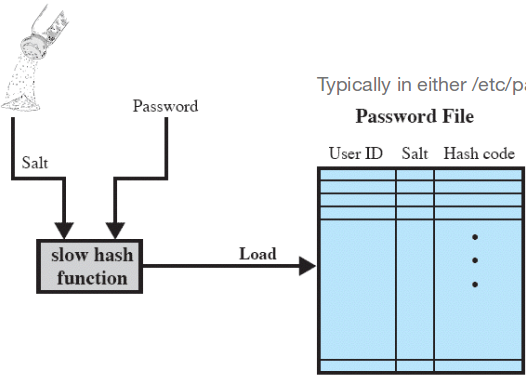
\includegraphics[scale=0.3]{salt1.png}\quad
\vline
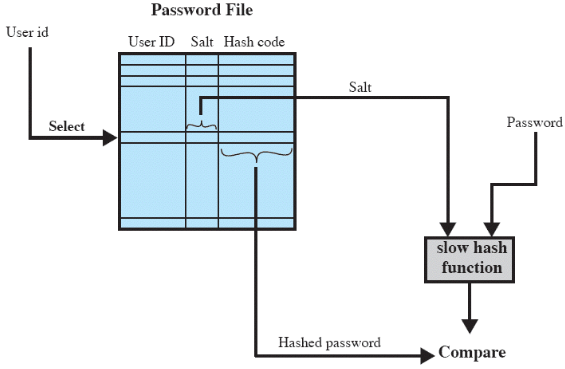
\includegraphics[scale=0.3]{salt2.png}

\end{frame}
%-----------------------------------------------------------------
\section{Linux Authentication}
\begin{frame}
\frametitle{Linux Authentication}
/etc/passwd\\
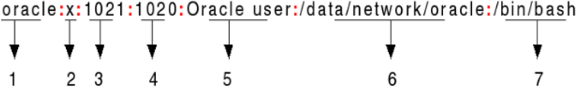
\includegraphics[scale=0.35]{pword.png}
\begin{enumerate}
\item Username - should be between 1-32 characters in length
\item Password - An x character the password is stored in file \texttt{/etc/shadow}
\item User ID (UID) - Each user must have have an assigned UID (0-999 are reserved).
\item Group ID (GID) - Users primary GID (stored in file \texttt{/etc/group}
\item User ID info - Comment field
\item Home Directory - absolute path to the directory the user will be in when they log in
\item Command/Shell - absolute path to a command or shell (e.g. \texttt{/bin/bash}
\end{enumerate}
\end{frame}
%--------------------------------------------------------------------
\section{Encryption}
\begin{frame}
\frametitle{Encryption}
\begin{itemize}
\item Hashed form generated by a ``one-way" function
\begin{itemize}
\item A one-way function that is easy to compute on every input, but hard to invert given the image of a random input
\item Here ``easy" and ``hard" are to be understood in the sense of computational complexity.
\item There are several candidates for ``one-way" functions. A common approach is based on multiplication and factorization
\item To factor 232-digit number (RSA-76A) took two years (100s of machines) in 2009.
\end{itemize}
\item Making the cryptographic hash function ``slow" to execute improves robustness against attack
\item As does enforcing a delay before passwords can be re-entered
\end{itemize}
\end{frame}
%--------------------------------------------------------------------
\section{Other methods}
\subsection{Zero-Knowledge Authentication}
\begin{frame}
\frametitle{Zero-Knowledge Autgentication}
\begin{itemize}
\item Solves problems inherent in password authentication
\item The user knows some ``secret" but must prove they know the secret without ever revealing it
\item The system verifies the user knows the secret without having to learn the secret
\item Since the secret is never revealed this method is zero-knowledge verification/authentication.
\end{itemize}
\end{frame}
%------------------------------------------------------------------
\section{Intrusion Detection}
\begin{frame}
\frametitle{Intrusion Detection}
\begin{itemize}
\item A specialist software layer designed to detect abnormal patterns of behaviour.
\item Sensors collect data describing behaviour patterns
\item Statistical analysis is used to determine likelihood of attempted unauthorised access
\item All multi-user systems maintain audit records activity logs; who performed what action with a particular object
\item Typically an audit record might contain subject, action, object, exception thrown, resource usage, time-stamps
\end{itemize}
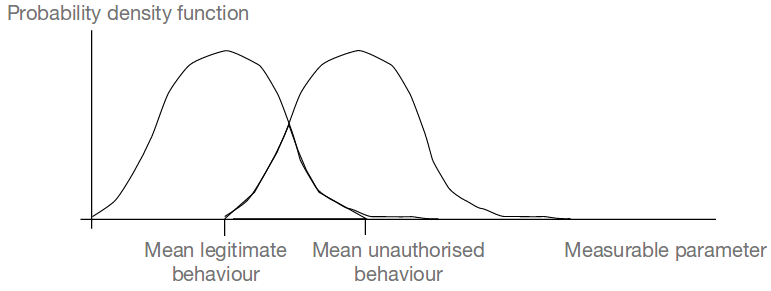
\includegraphics[scale=0.35]{id.png}
\end{frame}

%-------------------------------------------------------------------
\section{Access Control Matrices}
\begin{frame}
\frametitle{Access Control Matrices}
\begin{itemize}
\item File access controlled by 2D array:
\begin{itemize}
\item Rows list users
\item Cols list files
\end{itemize}
\item Set row/col cell to 1 if user is allowed access
\item Allows access to be set on individual files
\item Matrix is very large for large file systems
\item Set permissions on a wider scale using user classes typically three groups:
\begin{itemize}
\item User/Owner, groups, everyone else (world)
\end{itemize}
\end{itemize}
\end{frame}
%------------------------------------------------------------------
\section{Summary}
\begin{frame}
\frametitle{Summary}
\begin{itemize}
\item Security is vital at all levels of a system if any comoponent is compromised the the whole system could be compromised
\item Password authentication can combat eavesdropping
\item Intrusion detection looks for unusual patterns of behaviour threshold setting can be a challenge
\item Authorisation is enforced by access control mechanisms
\end{itemize}
\end{frame}
%------------------------------------------------------------------

\begin{frame} 
\Huge{\centerline{The End}}
\end{frame}

\end{document}